
Die Detaillierung des Entwurfes basiert größtenteils auf Maßen verfügbarer Kaufteile und Abschätzungen für gewählte Abmessungen anhand von Ausführungen oder Beispielen in den herangezogenen Veröffentlichungen. Dabei sind vor allem~\cite{Design_of_shielded_enclosures, EMV-gerechtes_Geraetedesign, EM_Schirmung, Simplified_shielding, Handbook_Shielding_Materials_and_Performance} zu nennen, die als Referenz für Abschätzungen dienten. Die folgenden Ausführungen schildern das Ergebnis des Konstruktionsprozesses in einer möglichst systematischen Reihenfolge.

\subsection{Verwendete Messtechnik}

Die Hauptkomponente der verwendeten Messtechnik stellt, wie bereits erwähnt, ein \ac{VNA} dar. Der für diese Arbeit zur Verfügung stehende \ac{VNA} der Firma Anritsu ist ein Zweikanal-Netzwerkanalysator mit einem Arbeitsbereich zwischen \SI{1}{\mega\hertz} und \SI{20}{\giga\hertz}. Ein Auszug mit den für dieses Modell relevanten Daten und Diagrammen nach~\cite{VNA-Datenblatt} ist im \Anhang\ref{A:Datenblatt_VNA} zu finden. 
\par
\vspace{\linespace}
Da der \ac{VNA} mithilfe der zwei verfügbaren Ports sowohl die Sendeantenne speist, als auch das Messsignal an der Empfangsanatenne aufnimmt, kann die Ermittlung der Schirmdämpfung direkt von der zugehörigen Software erfolgen. Außerdem sind sogenannte Zeitbereichsmessungen (Time Domain Measurements) möglich, wodurch eine Unterscheidung zwischen dem direkten und indirekten Koppelpfad möglich ist~\cite{Techniques_Shielding_Effectiveness_Far_Field_Simulation}. Im \Kapitel\ref{cha:4} wird darauf näher eingegangen.
\par
\vspace{\linespace}
Die Kalibration der Messtechnik erfolgt mithilfe des zugehörigen Kalibrationskits, wodurch bei korrekter Durchführung die im Auszug des Datenblattes (vgl. \Anhang\ref{A:Datenblatt_VNA}) dargestellten Unsicherheiten eingehalten werden sollten. Die durchgeführte Kalibration des \ac{VNA} wird im \Abschnitt\ref{cha:4_Kalibration_Messtechnik} ausführlich dargestellt.
\par
\vspace{\linespace}
Der \ac{VNA} soll mittels der ebenfalls zugehörigen Signalkabel, die eine Wellenimpedanz von \SI{50}{\ohm} aufweisen, mit den Antennen verbunden werden~\cite{Testkabel_VNA-Datenblatt}. Die Anschlüsse sind \ac{SMA} kompatible Steckverbinder mit \SI{2,92}{\milli\meter}-Stecker.
\par
\vspace{\linespace}
%Antennen/Waveguides
    %Größe
    %Platziert mit vorhandenen Stativen
Die zur Verfügung stehenden Antennen sind Breitband-Hornstrahler mit einer linearen Polarisation und den in der \Tabelle\ref{tab:3_Spezifikationen_Antennen} zusammengefassten wichtigstens Spezifikationen nach~\cite{Antennen-Datenblatt}. Weitere Kenndaten sind im \Anhang\ref{A:Datenblatt_Antennen} zu finden. Die Antennen bieten ebenfalls einen SMA-Anschluss für die Signalkabel.

\begin{table}[ht]
    \centering
    \caption{Technische Spezifikationen der verwendeten Hornstrahler nach~\cite{Antennen-Datenblatt}}
    \label{tab:3_Spezifikationen_Antennen}
    \begin{tabular}{p{6cm} C{5cm}}
    \toprule
        \textbf{Spezifikation} & \textbf{Wert} \\
    \midrule
        Frequenzbereich & $0,8 - 18\;\si{\giga\hertz}$ \\
        Halbwerts-Strahlbreite  & $111-13 \;\si{\degree}$ (E-Feld) \\
                                & $78-10\;\si{\degree}$ (H-Feld) \\
        Kreuzpolarisation-Isolation & \SI{25}{\Dezibel} (typ.) \\
        Stehwellenverhältnis (VSWR) & $1,5 : 1$ (typ.) \\
        Abmessungen             & $244\times160,5\times228\;\si{\milli\meter}$ \\
    \bottomrule
    \end{tabular}
\end{table}

Mithilfe der zugehörigen Aluminium-Stative können die Antennen frei auf einer Höhe zwischen \SI{53}{\centi\meter} und \SI{158}{\centi\meter} platziert werden.




\subsection{Konstruktion}

Die Modulwände werden hauptsächlich aus den Sandwichpaneelen gebildet, wodurch die Auswahl dieser von zentraler Bedeutung für die restliche Konstruktion ist. Aufgrund von Produktverfügbarkeiten mussten Verbundplatten aus Sperrholz mit metallischen Deckblechen, wie sie im Rahmen professioneller Absorberkammern zum Einsatz kommen, schon zu Beginn der Konzeptphase verworfen werden. Als Alternative wurden Wabenkernplatten gewählt, die ebenfalls durchgehende Deckbleche besitzen, aufgrund der inneren Struktur ein deutlich günstigeres Verhältnis aus Biegesteifigkeit und Gewicht besitzen und auf ganz ähnliche Weise verarbeitet werden können~\cite{Alucore-Datenblatt}. Im Messbereich zwischen $1\ldots18\;\si{\giga\hertz}$ ist nach \Abschnitt\ref{cha:2_sub_Schirmung_ebener_Wellenfelder} die Absorptions- und Reflektionsdämpfung für die kombinierten \SI{2}{\milli\meter} Blechstärke bereits so hoch, dass für die real erreichte Schirmung des Versuchsstandes gegenüber Störquellen von außen nur noch Öffnungen wie Türen oder Verbindungsstellen entscheident sind.  
\par
\vspace{\linespace}
Für den vorgesehenen Einsatzzweck musste die Polyesterlackschicht an allen Wirkflächen, das heißt allen Verbindungsflächen der Modulwände untereinander und allen weiteren Anschlussflächen, mechanisch entfernt werden. Um trotz der sich stets an Luftatmosphäre bildenden Oxidschichten einen leitfähigen Kontakt an allen Wirkflächen herzustellen, werden Funktionselemente nach Möglichkeit miteinander verschraubt. Dabei kann im Fall von Aluminium bereits bei kleinen Vorspannkräften im Bereich von \SI{1000}{\newton} davon ausgegangen werden, dass die harten Oxidschichten aufreißen und Metall-Metall-Kontakt entsteht~\cite{Projektarbeit}. Im Fall der Türdichtungen gewährleisten die gewählten HF-Dichtungen aufgrund der Relativbewegung bei jedem Schließvorgang eine mechanische Entfernung der Oxidschichten.
\par
\vspace{\linespace}
Die Grundlage für die Auslegung der L-Profile bildet der aus der Schraubenberechnung bekannte Rötscher-Kegel. Die Schenkellänge der Profile, welche die Wabenkernplatten an den Eckstößen miteinander verbinden, wurden entsprechend der verfügbaren Profilmaße so gewählt, dass sich der Verspannungskegel innerhalb der verschraubten Teile vollständig ausbilden kann und somit die Vorspannkraft der Schrauben möglichst großflächig in die Wabenkernplatte eingeleitet wird. Die \Abb\ref{fig:3_Verspannungskegel_L-Profile} zeigt dies in einer schematischen Darstellung zusammen mit den gewählten Profilmaßen und dem sich ergebenden Ersatzquerschnitt des Schraubverbandes. 

\begin{figure}[ht]
    \centering
    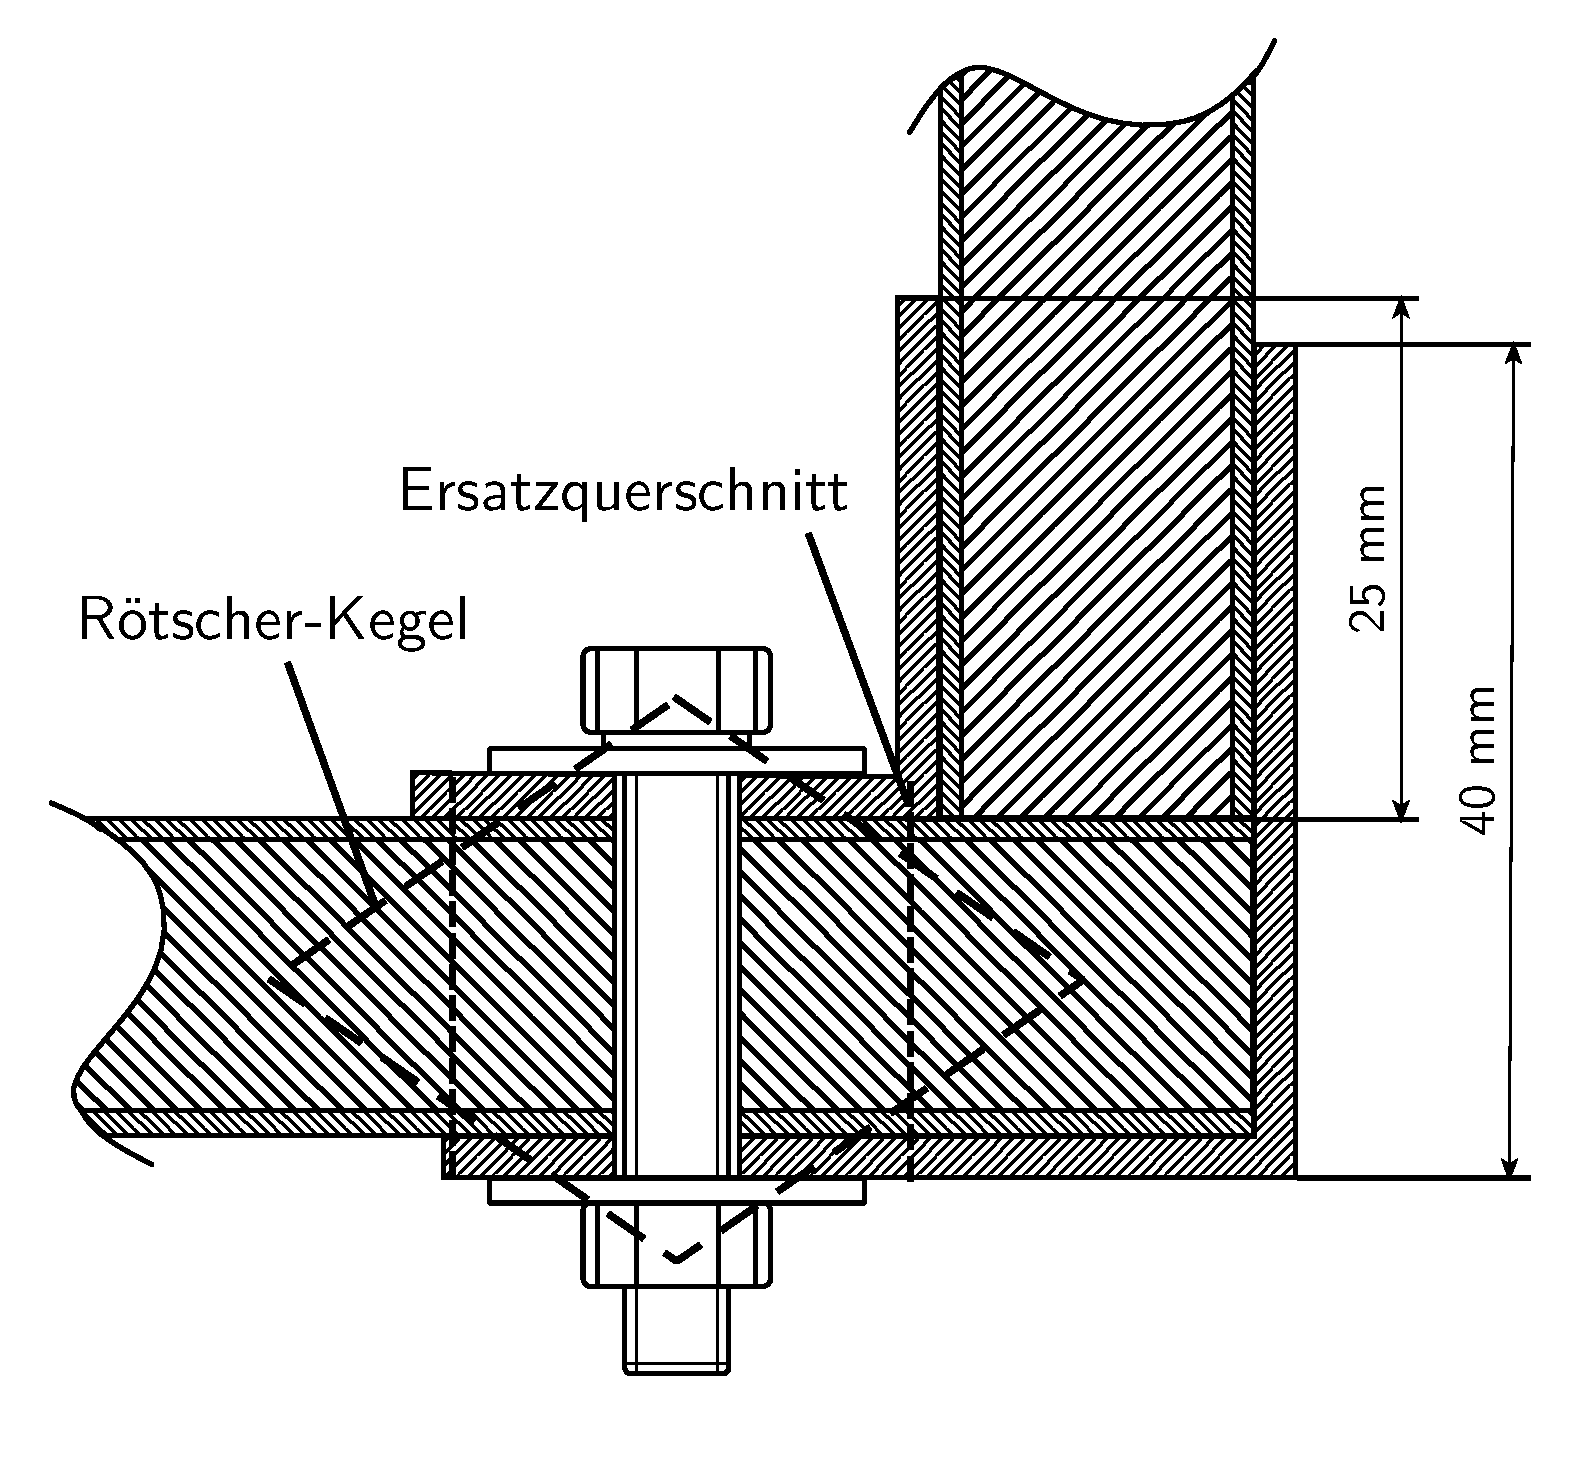
\includegraphics[page=1, trim=0cm 0cm 0cm 0cm, clip, width = .45\textwidth]{Abbildungen/Kapitel3/Schematik_Verspannungskegel.pdf}
    \caption{Schematische Darstellung des Verspannungsbereiches der verschraubten Modulwände}
    \label{fig:3_Verspannungskegel_L-Profile}
\end{figure}


Die Wahl des Schraubenabstandes wurde auf Grundlage eines Zusammenhanges nach~\cite{Design_of_shielded_enclosures} getroffen, welcher die erreichbare Schirmdämpfung als Funktion des Schraubenabstandes verschraubter Blechteile darstellt. Wie aus der Grafik in \Abb\ref{fig:3_Schirmwirkung_Schraubenabstand} hervorgeht, kann bei einem Schraubenabstand von \SI{10}{\centi\meter} von etwa \SI{70}{\Dezibel} theoretisch erreichbarer Schirmdämpfung je Funktionsfläche ausgegangen werden. Dieser Abstand wurde auch in Hinblick auf den Fertigungsaufwand der Bohrungen und Verschraubungen gewählt. Aufgrund der Sandwichbauweise der Modulwände befinden sich des Weiteren stets zwei Wirkflächen im Koppelpfad, wodurch der Durchgriff weiter verringert wird. Die Anfertigung der Bohrungen erfolgte händisch und während des Zusammenbauprozesses, um eine möglichst exakte Ausrichtung der Bohrlöcher in den einzelnen verspannten Teilen relativ zueinander zu erreichen.  


\begin{figure}[ht]
    \centering
    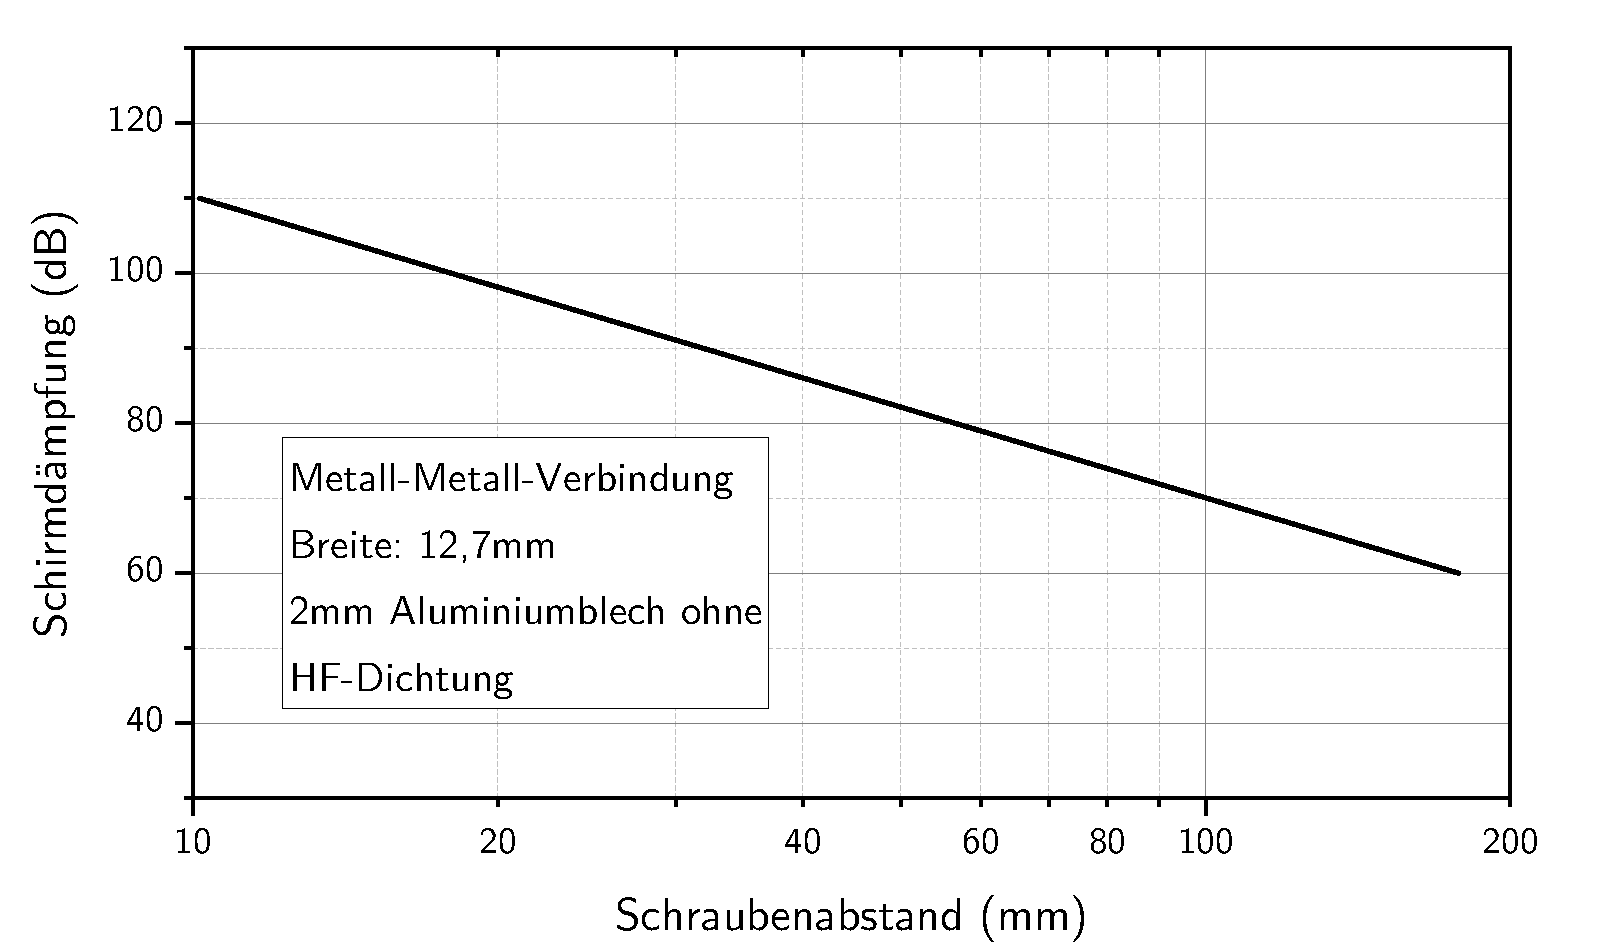
\includegraphics[page = 1, trim = 0cm 0cm 0cm 0cm, clip, width=.65\textwidth]{Abbildungen/Kapitel3/Schraubenabstand_Schirmwirkung.pdf}
    \caption[Schirmdämpfung verschraubter Blechteile in Abhängigkeit des Schraubenabstandes]{Schirmdämpfung verschraubter Blechteile in Abhängigkeit des Schraubenabstandes nach~\cite{Design_of_shielded_enclosures}}
    \label{fig:3_Schirmwirkung_Schraubenabstand}
\end{figure}

\par
\vspace{\linespace}
Um eine möglichst hohe Schirmdämpfung zu erreichen, wurde die Anordnung der Profile mit entsprechenden Aussparungen so gewählt, dass sich an keiner Stelle zwei Anschlussstellen direkt gegenüberstehen. Dies führt zu einer Labyrinthwirkung an Stellen von Profilübergängen und verringert somit ebenfalls den Felddruchgriff an den Kontaktstellen der Profile. Mit dem gewählten Konzept wäre eine höhere Schirmwirkung an den Verbindungsstellen der Profile untereinander nur durch dichtes Verschweißen oder Verlöten zu erreichen~\cite{Design_of_shielded_enclosures, EM_Schirmung}. 
\par
\vspace{\linespace}


%Wabenkernplatten als Grundlage 
    %Verfügbarkeit
    %Vorteile gegenüber Vollmaterial (ggf. mit Grafik bzw. Wert
    %Datenblatt ggf. einfügen
    %Besonderheiten (Entfernen der Lackschicht z.B.)
    
%Aluprofile mit Rechnung bzw. der gewählten Dicke und Maßen

%Schraubenberechnung ggf.

%(Aufbau-(Reigenfolge))




Die Auswahl geeigneter Absorberelemente zur Reduktion von Reflektionen und Vermeidung von Hohlraumresonanzen in der Messkabine wurde unter Einbeziehung der erreichbaren Reflektionsdämpfung, der Höhe einzelner Elemente und ökonomischen Gesichtspunkten getroffen. Die Reflektionsdämpfung gibt hierbei das Verhältnis einer eintreffenden Welle zum reflektierten Anteil an. Eine möglichst hohe und gleichbleibende Reflektionsdämpfung über alle Einsatzfrequenzen ist dementsprechend wünschenswert. Im \Abschnitt\ref{cha:3_Entwurf} wurde die Auswahl bereits auf reine Pyramidenabsorber eingeschränkt. Zur Vermeidung von reflektivem Verhalten bei hohen Frequenzen wurde auf Absorberelemente mit abgeschnittener Spitze verzichtet. 
\par
\vspace{\linespace}
Die gewählten Absorber besitzen die in \Tabelle\ref{tab:3_Reflektionsdaempfung_Absorberelemente} angegebene garantierte Reflektionsdämpfung im Messbereich dieser Arbeit. Mit einer Höhe von \SI{10}{\centi\meter}  verbleibt auch nach dem Einbau noch ein großer Messbereich in der Testkammer. Des Weiteren ist vor allem im höheren Frequenzbereich eine höhere Reflektionsdämpfung zu erwarten, als bei der \SI{20}{\centi\meter} hohen Variante der gleichen Produktfamilie. Auf die Verwendung noch höherer Elemente wurde aufgrund der steigenden Einschränkung des Messraumes und ökonomischer Sicht verzichtet.  


\begin{table}[ht]
    \centering
    \begin{tabular}{p{2cm} C{1.6cm} C{1.6cm} C{1.6cm} C{1.6cm} C{1.6cm}}
        \toprule
            &   \multicolumn{5}{l}{\textbf{Reflektionsdämpfung [\SI{}{\Dezibel}]}} \\
        \midrule
            &   \SI{1}{\giga\hertz} & \SI{3}{\giga\hertz} & \SI{5}{\giga\hertz} & \SI{10}{\giga\hertz} & \SI{18}{\giga\hertz} \\
        \textbf{Gemessen}   &   15  &   32  &   42  &   50  &   55 \\    
        \textbf{Garantiert} &   12  &   30  &   40  &   45  &   50 \\
        \bottomrule
    \end{tabular}
    \caption[Gemessene und garantierte Reflektionsdämpfung der verwendeten EPP12 Pyramidenabsorber im Bereich zwischen \SI{1}{\giga\hertz} bis \SI{18}{\giga\hertz}]{Gemessene und garantierte Reflektionsdämpfung der verwendeten EPP12 Pyramidenabsorber im Bereich zwischen \SI{1}{\giga\hertz} bis \SI{18}{\giga\hertz} nach~\cite{Eco_Messtechnik_Absorber}}
    \label{tab:3_Reflektionsdaempfung_Absorberelemente}
\end{table}

Auf dem Messprotokoll~\cite{Eco_Messtechnik_Absorber} sind außerdem keine ausgezeichneten Peaks des Dämpfungsverhaltens zu erkennen. In Bezug auf Kosten und Höhe vergleichbare alternative Absorber bieten ab etwa \SI{5}{\giga\hertz} nur eine um \SI{5}{\Dezibel} reduzierte Reflektionsdämpfung, was bei Betrachtung des Verhältnisses der Feldgrößen etwa einem Faktor 2 entspricht (vgl. \Tabelle\ref{tab:2_Relative_Pegel})~\cite{Holland_Shielding_Absorber}. Mit Ferritkacheln und zusätzlich darauf abgestimmten Hybridabsorbern kann zwar bereits im Frequenzbereich zwischen \SI{1}{\giga\hertz} bis \SI{3}{\giga\hertz} eine Reflektionsdämpfung von \SI{25}{\Dezibel} erreicht werden, jedoch ist mit dieser Kombination aufgrund der Impedanzabstimmung der PU-Absorber auf die Ferritkacheln bei hohen Frequenzen nur mit etwas mehr als \SI{30}{\Dezibel} zu rechnen, ab \SI{10}{\giga\hertz} sogar nur mit weniger als \SI{30}{\Dezibel}~\cite{Holland_Shielding_Absorber}, mit teils stark ausgeprägten Peaks in bestimmten Frequenzbändern. Aus diesen Gründen wurden die oben beschriebenen Absorber des Types EPP12 der Firma \Firma{ECO-Messtechnik GmbH und Co. KG} verwendet, die außerdem nach DIN 4102 als nicht brennbar der Klasse M2 (CSTB) eingestuft wurden~\cite{Eco_Messtechnik_Absorber}. 
\par
\vspace{\linespace}
Da aufgrund der Höhe der Pyramidenabsorber keine exakte Auskleidung der Schnittstellen zwischen den Modulwänden erfolgen kann, wurden zusätzliche Flachabsorber des Types EPF15, welche ebenfalls von \Firma{ECO-Messtechnik GmbH und Co. KG} angeboten werden~\cite{Eco_Messtechnik_Absorber}, an den Ecken des Versuchsstandes angebracht. Die Befestigung der Absorberelemente erfolgte mittels Klettbändern, um eine nachträgliche Justierung oder einen Austausch zu ermöglichen.   
\par
\vspace{\linespace}

%Absorberelementauswahl 
    %Datenblatt
    %Anzahl Abschätzung
    %Flachabsorber für Ecken
    %Befestigung
    




    
%Probenreflektor mit Probenhalterung (CAD ggf.) und Beschreibung der Probenhalterung mit Vorteil der verschiedenen Dicken der Probekörper

%ggf. Prositionierung der Antennen (Stativ aus Holz)

%Türen mit Verschlüssen
    %Begründung Anzahl Verschlüsse
    %Detail mit Abstandshalter der Scharniere (damit Kontaktfederstreifen nicht zusammengedrückt werden)

%Auswahl Kabeldurchführungen (Impedanz von 50 Ohm im Match mit VNA --> Verweis Datenblatt VNA und Kabeldurchführungen (Muss matchen, um keine Rückreflektion zu bekommen (siehe Folien von Connector Care))
    %ggf. Detail mit Kupferplatte hierhin und nicht in Entwurf
    




